\chapter{MATEMATIČKA POZADINA STATISTIČKE PIV EVALUACIJE}
\label{chap:Poglavlje_3}
U ovom poglavlju prikazan je pojednostavljeni opis matematičkog modela snimanja, te statističke evaluacije PIV snimki. Analizirana je kros-korelacija na dva kadra (snimke), svaka snimka je izložena jednoj ekspoziciji. Matematičku teoriju evaluacije više-ekspozicioniranih snimki moguće je pronaći u literaturi \cite{raffel2018_book}.
\section{Položaj čestica na snimkama}
PIV snimke su tijekom evaluacije podijeljene na prozore ispitivanja. Važno je napomenuti kako su PIV snimke 2-dimenzionalne, dok osvijetljena laserska ploha ima određenu debljinu (treću dimenziju). Geometrijska projekcija PIV slika na lasersku osvijetljenu ravninu prikazana je na \textit{Slici \ref{sl:3.1}}.
\begin{figure}[h]  
	\centering
	%\usepackage{graphicx}
	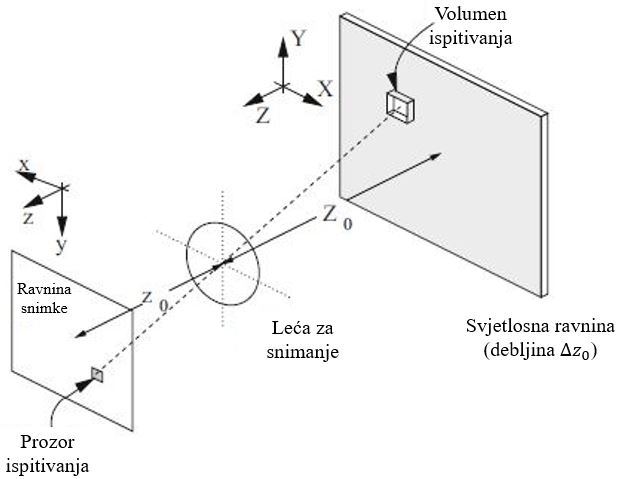
\includegraphics[width=11cm]{./3_MatPozadina/3_1ShemaPIVsnimki.jpg} 
	\caption{Shematski prikaz geometrije snimanja\cite{raffel2018_book}}
	\label{sl:3.1}
\end{figure}
\par
Neka se razmatra snimka pri jednoj ekspoziciji. Na snimci se nalaze slučajno distribuirane slike čestica, koje odgovaraju $N$ broju čestica markera ubačenih u strujanje:
\begin{equation}
	\boldsymbol{\Gamma} = \left[ \begin{array}{c}
						\boldsymbol{X_{1}} \\
						\boldsymbol{X_{2}} \\
						\vdots \\
						\boldsymbol{X_{N}}
					\end{array} \right]
\label{eqn:3.1}
\end{equation}
gdje je $\boldsymbol{X_{i}}=\left(X_{i}, Y_{i}, Z_{i}\right)$ vektor pozicije čestice $i$ u trenutku $t$. $\boldsymbol{\Gamma}$ opisuje stanje cjeline u trenutku $t$. Jednadžba \ref{eqn:3.1} označava poziciju čestica u 3D prostoru (volumena ispitivanja). Malim slovim će se označavati koordinate čestica na ravnini snimke (\textit{Slika \ref{sl:3.1}}) tako da $x$ označava poziciju čestice na snimci:
\begin{equation}
	\boldsymbol{x} = \left[ \begin{array}{c}
		x\\
		y
	\end{array}\right]
\label{eqn:3.2}
\end{equation}
Radi jednostavnosti pretpostavit će se kako su pozicije čestica u volumenu ispitivanja i njene pozicije u ravnini snimke povezane konstantnim faktorom povećanja $M$ tako da vrijedi:
\begin{equation}
	\boldsymbol{X_{i}}=\dfrac{\boldsymbol{x_{i}}}{M} \quad\text{i}\quad \boldsymbol{Y_{i}}=\dfrac{\boldsymbol{y_{i}}}{M}
\label{eqn:3.3}
\end{equation}
\FloatBarrier
\section{Polje intenziteta snimke}
U ovom dijelu prikazan je intenzitet distribucije vrijednosti u ravnini snimke. Pretpostavlja se kako snimka najbolje može biti opisana konvolucijom geometrijske slike i impulsnog odziva sustava snimanja, tkv. funkcijom širenja točke PSF (\textit{eng. point spread function}) \cite{raffel2018_book}. PSF se u mnogim kontekstima može smatrati proširenom mrljom jedne čestice (\textit{Slika \ref{sl:3.2}}), to jest mjerom koliko će se točka (čestica) proširiti zbog loše kvalitet sustava snimanja \cite{wiki:Point_spread_function}. Za infinitezimalno malenu česticu i bez aberacije fokusiranu leću, amplituda PSF-a matematički je opisana Airy-ovom funkcijom (Bessel-ova funkcija prvog reda).
\begin{figure}[h]  
	\centering
	%\usepackage{graphicx}
	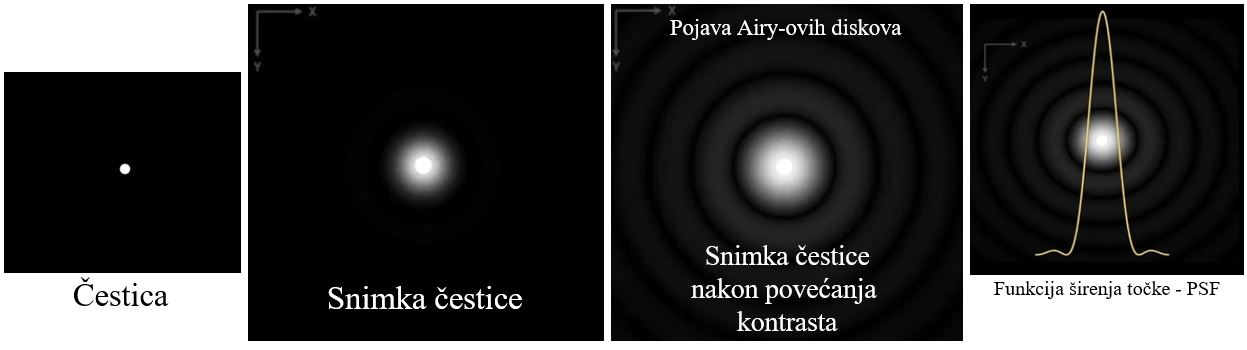
\includegraphics[width=15cm]{./3_MatPozadina/3_2PSF.jpg} 
	\caption{PSF i pojava Airy-ovih diskova \cite{youtube_PSF}}
	\label{sl:3.2}
\end{figure}
\par
U ovoj analizi pretpostaviti će se da funkcija širenja točke PSF leće za snimanje $\tau (\boldsymbol{x})$ ima sličan oblik Gauss-ovoj funkciji, što je uobičajena praksa i dobra aproksimacija za PSF leće za snimanje u stvarnom slučaju:
\begin{equation}
	\tau (\boldsymbol{x}) = K \, \exp \left(-\dfrac{8|\boldsymbol{x}|^2}{d_{\tau}^{2}}\right)
	\label{eqn:3.4}
\end{equation}
gdje je:
\begin{equation*}
	K = \dfrac{8\tau_{0}}{\pi d_{\tau}^{2}}
\end{equation*}
$d_{\tau}$ predstavlja razliku između stvarnog i idealnog promjera čestice na snimci. Konvolucijski produkt $\tau (\boldsymbol{x})$ sa geometrijskom slikom čestice markera na poziciji $\boldsymbol{x_{i}}$ opisuje položaj jedne čestice na poziciji $\boldsymbol{X_{i}}$. Nadalje, analiza će se ograničiti na infinitezimalno male geometrijske slike čestica, što je inače slučaj kod snimanja malenih čestica na malim uvećanjima. Stoga se koristi Dirac delta-funkcija pomaknuta na poziciju $\boldsymbol{x_{i}}$ kako bi se opisao geometrijski dio slike čestice. Na ovaj način polje intenziteta snimke (\textit{Slika \ref{sl:3.3}}) prilikom jedne ekspozicije može biti dano izrazom:
\begin{equation}
	I = I (\boldsymbol{x}, \boldsymbol{\Gamma}) = \tau (\boldsymbol{x}) \ast \sum_{i=1}^{N}V_{0}(\boldsymbol{X_{i}}) \, \delta (\boldsymbol{x}-\boldsymbol{x_{i}})
	\label{eqn:3.5}
\end{equation}
gdje je $V_{0} (\boldsymbol{X_{i}})$ transfer funkcija koja je dana energijom svijetla slike jedne čestice $i$ unutar volumena ispitivanja $V_{I}$  i njenom konverzijom u električni signal. $\tau (\boldsymbol{x})$ se smatra identičnim za svaku poziciju čestice. Vidljivost čestice ovisi o mnogo parametara, a jedni od važnijih su: svojstvo čestice da raspršuje svjetlost, jačina svjetlosti na mjestu gdje se nalazi čestica, osjetljivost optike za snimanje, kvaliteta senzora na kameri. Ovdje će se pretpostaviti kako čestice na svakoj poziciji imaju ista svojstva raspršivanja, te ostala tehnika za snimanje također ima ista svojstva. Potrebno je napomenuti kako u slučaju različitih svojstava, moguće je množenje različitih prozora ispitivanja za različitim kernelima koji će ta svojstva "ispeglati".
\begin{figure}[h]  
	\centering
	%\usepackage{graphicx}
	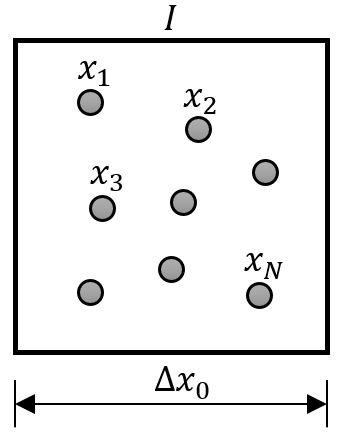
\includegraphics[width=3cm]{./3_MatPozadina/3_3primjerPoljaCestica.jpg} 
	\caption{Primjer polja $I$ prilikom samo jedne ekspozicije}
	\label{sl:3.3}
\end{figure}
\par
Nadalje, neka $Z$ predstavlja smjer gledanja, intenzitet svjetla unutar područja ispitivanja je tako jedino u funkciji $Z$ i na kraju analizirani intenzitet snimke jedino ovisi o $X$ i $Y$. Stoga, $V_{0} (\boldsymbol{X})$ opisuje oblik, produženje i lokaciju stvarnog volumena ispitivanja.
\begin{equation}
	V_{0}(\boldsymbol{X}) = W_{0}(X, Y)\, I_{0}(Z)
	\label{eqn:3.6}
\end{equation}
gdje je $I_{0}(z)$ profil intenziteta laserske zrake u $Z$ smjeru, a $W_{0}(X, Y)$ funkcija prozora ispitivanja geometrijski projicirana na svjetlosnu ravninu. Treba napomenuti kako ovo matematički nije točno zbog toga što nije uzeta u obzir konvolucija sa funkcijom širenja točke PSF. Samim time može se zaključiti kako za prozore ispitivanja u obliku pravokutnika u prikazanom matematičkom opisu zanemaren je efekt djelomično obrezanih (\textit{eng. cropped}) snimki na rubovima područja ispitivanja. Međutim, ovaj jednostavni model prozora ispitivanja će se koristiti u strujanju zbog toga što pojednostavljuje opis PIV evaluacije. Izraz
\begin{equation}
	I_{o}(Z) = I_{Z}\, \exp\left(-8\dfrac{(Z-Z_{0})^{2}}{\Delta Z_{0}^{2}}\right)
	\label{eqn:3.7}
\end{equation}
će se korisiti kako bi se opisao Gauss-ov profil intenziteta u $Z$ smjeru laserske svjetlosne ravnine. $\Delta Z_{0}$ predstavlja debljinu svjetlosne ravnine, a $I_{Z}$ je maksimalna vrijednost intenziteta svjetlosne ravnine. Funkcija $W_{0}(X, Y)$ također je opisana Gauss-ovom funkcijom u kojoj uzimamo u obzir maksimalni težinski faktor $W_{XY}$ na poziciji $X_{0}$, $Y_{0}$:
\begin{equation}
	W_{0}(X, Y)=W_{XY}\, \exp \left(-8\dfrac{(X-X_{0})^{2}}{\Delta X_{0}^{2}}-8\dfrac{(Y-Y_{0})^{2}}{\Delta Y_{0}^{2}}\right)
	\label{eqn:3.8}
\end{equation}
Osim Gauss-ovom funkcijom, intenzitet distribucije laserske ravnine može (jednostavnije) biti opisan i sa top-hat funkcijom. U tom slučaju $I_{0}(Z)$ i $W_{0}(X, Y)$ imaju oblik:
\begin{equation}
	I_{0}(Z))=\begin{cases}
		I_{Z} &\text{ako je}\quad |Z-Z_{0}|\leq \dfrac{\Delta Z_{0}}{2}\\
		0 &\text{inače}
	\end{cases}
	\label{eqn:3.9}
\end{equation}
\begin{equation}
	W_{0}(X, Y))=\begin{cases}
		W_{XY} &\text{ako je}\quad |X-X_{0}|\leq \dfrac{\Delta X_{0}}{2}\quad \text{i}\quad |Y-Y_{0}|\leq \dfrac{\Delta Y_{0}}{2}\\
		0 &\text{inače}
	\end{cases}
	\label{eqn:3.10}
\end{equation}
Faktor $I_{0}(Z_{i})$ predstavlja primljenu količinu svjetla od čestice $i$ unutar strujanja lociranu na udaljenosti $|Z_{i}-Z{0}|$ od središnje ravnine laserske plahte. $\Delta Z_{0}$ je debljina laserske ravnine (ekstenzija volumena ispitivanja u $Z$ smjeru), dok su $\Delta X_{0}=\Delta x_{0}/M$ i $\Delta Y_{0}=\Delta y_{0}/M$ ekstenzije volumena ispitivanja u $X$ i $Y$ smjeru. Ako je funkcija širenje točke (PSF) $\tau (\boldsymbol{x}-\boldsymbol{x_{i}})=\tau \ast \delta (\boldsymbol{x}-\boldsymbol{x_{i}})$ i ako se uzme pretpostavka da promatrane snimke čestica se ne preklapaju jednažba \ref{eqn:3.5} alternativno se može zapisati:
\begin{equation}
	I(\boldsymbol{x}, \boldsymbol{\Gamma})=\sum_{i=1}^{N}V_{0}(\boldsymbol{X_{i}})\, \tau (\boldsymbol{x}-\boldsymbol{x_{i}})
	\label{eqn:3.11}
\end{equation}
Jednadžba \ref{eqn:3.11} predstavlja polje intenziteta snimke, te će ovaj izraz biti korišten u opisu korelacije dane primjerom sa tri proizvoljno pozicionirane čestice.
\FloatBarrier
\section{Srednja vrijednost, auto-korelacija i varijanca jednom ekspozicionirane snimke}
U ovom dijelu prikazati će se pojmovi auto-korelacije i auto-kovarijance jednom ekspozicionirane snimke. Također, biti će određeni srednja vrijednost i varijanca, koje su bitne vrijednosti polja intenziteta snimke jer se uz pomoć njih vrši normalizacija kros-korelacije. Prostorni prosjek je definiran izrazom \cite{raffel2018_book}:
\begin{equation}
	\langle I(\boldsymbol{x}, \boldsymbol{\Gamma})\rangle =\dfrac{1}{a_{I}}\int_{a_{I}}I(\boldsymbol{x}, \boldsymbol{\Gamma})dx
	\label{eqn:3.12}
\end{equation}
gdje $a_{I}$ predstavlja područje ispitivanje. Uvrštavanjem jednadžbe \ref{eqn:3.11} u \ref{eqn:3.12} dobije se:
\begin{equation}
	\langle I(\boldsymbol{x}, \boldsymbol{\Gamma})\rangle =\dfrac{1}{a_{I}}\int_{a_{I}}\sum_{i=1}^{N}V_{0}(\boldsymbol{X_{i}})\, \tau (\boldsymbol{x}-\boldsymbol{x_{i}})dx
	\label{eqn:3.13}
\end{equation}
Srednja vrijednost polja intenziteta može biti aproksimirana sa:
\begin{equation}
	\mu_{I}=\langle I(\boldsymbol{x}, \boldsymbol{\Gamma})\rangle =\dfrac{1}{a_{I}}\sum_{i=1}^{N}V_{0}(\boldsymbol{X_{i}}\int_{a_{I}}\tau (\boldsymbol{x}-\boldsymbol{x_{i}}))dx
	\label{eqn:3.14}
\end{equation}
Sada je moguće izvesti auto-korelaciju jednom ekspozicioniranog polja intenziteta na sličan način:
\begin{equation}
	\begin{split}
		R_{I}(\boldsymbol{s}, \boldsymbol{\Gamma}) &= \langle I(\boldsymbol{x}, \boldsymbol{\Gamma})\, I(\boldsymbol{x}+\boldsymbol{s}, \boldsymbol{\Gamma})\rangle\\
		 &= \dfrac{1}{a_{I}}\int_{a_{I}}\sum_{i=1}^{N}V_{0}(\boldsymbol{X_{i}})\, \tau (\boldsymbol{x}-\boldsymbol{x_{i}})\sum_{j=1}^{N}V_{0}(\boldsymbol{X_{j}})\, \tau (\boldsymbol{x}-\boldsymbol{x_{j}}+\boldsymbol{s})dx
		 \label{eqn:3.15}
	\end{split}
\end{equation}
gdje $s$ predstavlja vektor separacije u korelacijskoj ravnini. Razlikovanjem $i\neq j$ članova koji predstavljaju korelaciju različitih snimki čestica, te samim time nasumično distribuirani šum u korelacijskoj ravnini od $i=j$ koji predstavljaju korelaciju svake čestice same sa sobom, izraz \ref{eqn:3.15} može se konačno zapisati kao:
\begin{equation}
	\begin{split}
		R_{I}(\boldsymbol{s}, \boldsymbol{\Gamma}) = &\dfrac{1}{a_{I}}\sum_{i\neq j}^{N}V_{0}(\boldsymbol{X_{i}})\, V_{0}(\boldsymbol{X_{j}})\int_{a_{I}}\tau (\boldsymbol{x}-\boldsymbol{x_{i}})\, \tau (\boldsymbol{x}-\boldsymbol{x_{j}}-\boldsymbol{s})dx\\
		 &+ \dfrac{1}{a_{I}}\sum_{i=j}^{N}V_{0}^{2}(\boldsymbol{X_{i}})\int_{a_{I}}\tau (\boldsymbol{x}-\boldsymbol{x_{i}})\, \tau (\boldsymbol{x}-\boldsymbol{x_{j}}-\boldsymbol{s})dx
	\end{split}
	\label{eqn:3.16}
\end{equation}
Jednadžbu \ref{eqn:3.16} moguće je raščlaniti i zapisati u obliku \cite{raffel2018_book}:
\begin{equation}
	R_{I}(\boldsymbol{s},\boldsymbol{\Gamma})=R_{C}(\boldsymbol{s},\boldsymbol{\Gamma})+R_{F}(\boldsymbol{s},\boldsymbol{\Gamma})+R_{P}(\boldsymbol{s},\boldsymbol{\Gamma})
	\label{eqn:3.17}
\end{equation}
gdje je: $R_{C}(\boldsymbol{s},\boldsymbol{\Gamma})$ kovolucija srednjih intenziteta $I$ (srednja pozadinska korelacija), $R_{F}(\boldsymbol{s},\boldsymbol{\Gamma})$ je fluktuirajuća komponenta šuma, te oba člana su rezultat $i\neq j$ članova. Dok, zadnji preostali član $R_{P}(\boldsymbol{s},\boldsymbol{\Gamma})$ predstavlja samo-korelacijski vrh na poziciji $(0, 0)$ u korelacijskoj ravnini i rezultat je $i=j$ članova (korelacija svih slika čestica samih sa sobom). Auto-korelacija podataka čestica sa snimke na \textit{Slici \ref{sl:3.3}} prikazana je na \textit{Slici \ref{sl:3.4}}, te jasno prikazan centralni korelacijski vrh $R_{P}$ i šum oko njega.
\begin{figure}[h]  
	\centering
	%\usepackage{graphicx}
	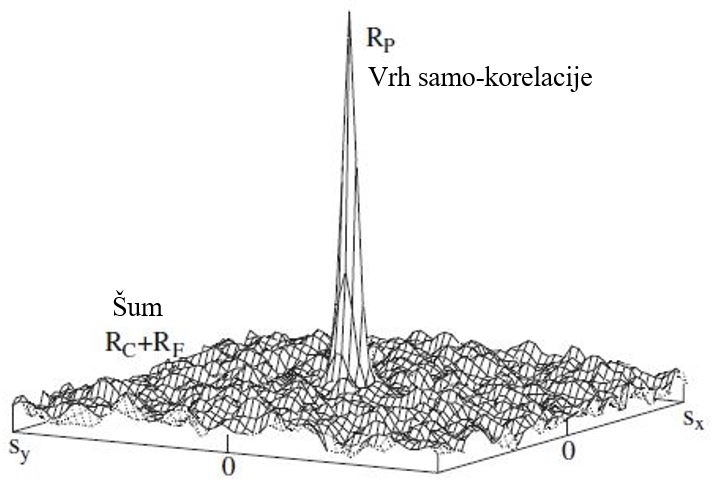
\includegraphics[width=9cm]{./3_MatPozadina/3_4AutoKorelacija.jpg} 
	\caption{Kompozicija vrhova u auto-korelacijskoj funkciji \cite{raffel2018_book}}
	\label{sl:3.4}
\end{figure}
\par
Ako auto-korelaciju sa \textit{Slike \ref{sl:3.4}} aproksimiramo Gauss-ovom funkcijom (jednadžba \ref{eqn:3.4}) koja ima širinu $\sqrt{2}d_{\tau}$ čime se zanemaruje šum, $R_{P}(\boldsymbol{s},\boldsymbol{\Gamma})$ se može zapisati kao:
\begin{equation}
	R_{P}(\boldsymbol{s},\boldsymbol{\Gamma}) = \sum_{i=1}^{N}V_{0}^{2}(\boldsymbol{X_{i}})\, \exp \left(\dfrac{-8|\boldsymbol{s}|^{2}}{d_{\tau}^{2}}\right)\dfrac{1}{a_{I}}\int_{a_{I}}\tau^{2}\left(\boldsymbol{x}-\boldsymbol{x_{i}}+\dfrac{\boldsymbol{s}}{2}\right)dx
	\label{eqn:3.18}
\end{equation}
U ovom radu korelacija snimke čestica $R_{\tau}(\boldsymbol{s})$ biti će prikazana izrazom:
\begin{equation}
	R_{\tau}(\boldsymbol{s})=\exp \left(\dfrac{-8|\boldsymbol{s}|^{2}}{d_{\tau}^{2}}\right)\dfrac{1}{a_{I}}\int_{a_{I}}\tau^{2}\left(\boldsymbol{x}-\boldsymbol{x_{i}}+\dfrac{\boldsymbol{s}}{2}\right)dx
	\label{eqn:3.19}
\end{equation}
pa samim time jednadžbu \ref{eqn:3.18} uvrštavanjem izraza \ref{eqn:3.19} može kraće zapisati kao:
\begin{equation}
	R_{P}(\boldsymbol{s},\boldsymbol{\Gamma})=R_{\tau}(\boldsymbol{s})\sum_{i=1}^{N}V_{0}^{2}(\boldsymbol{X_{i}})
	\label{eqn:3.20}
\end{equation}
Za polje intenziteta sa srednjom vrijednosti koja je jednaka nuli, auto-korelacija je jednaka auto-kovarijanci. Za ne-nula srednje vrijednosti polje intenziteta auto-kovarijance $C_{i}(s)$ može se dobiti izrazom \cite{raffel2018_book}:
\begin{equation}
	C_{I}(\boldsymbol{s})=R_{I}(\boldsymbol{s})-\mu_{I}^{2}
	\label{eqn:3.21}
\end{equation}
Procjena varijance tako ima oblik:
\begin{equation}
	\sigma_{I}^{2}=C_{I}(\boldsymbol{0}, \boldsymbol{\Gamma})=R_{I}(\boldsymbol{0}, \boldsymbol{\Gamma})-\mu_{I}^{2}=R_{P}(\boldsymbol{0}, \boldsymbol{\Gamma})-\mu_{I}^{2}
	\label{eqn:3.22}
\end{equation}
\FloatBarrier
\section{Kros-korelacija dvije uzastopne jednom ekspozicionirane snimke}
PIV snimke su obično evaluirane na način da se lokalno kros-koreliraju dvije uzastopne jednom ekspozicionirane snimke, te će u ovom potpoglavlju biti prikazan matematički opis spomenute kros-korelacije. Moguća je evaluacija i snimki koje su dva ili više puta ekspozicionirane (više u literaturi \cite{raffel2018_book}).\\
Za početak, potrebno je pretpostaviti vektor konstantnih pomaka $\boldsymbol{D}$ svih čestica unutar volumena ispitivanja, tako da se položaj čestica na snimici prilikom druge ekspozicije u trenutku $t' = t + \Delta t$ može zapisati kao:
\begin{equation}
	\boldsymbol{X_{i}^{'}}=\boldsymbol{X_{i}}+\boldsymbol{D}=\left[ \begin{array}{c}
																		X_{i}+D_{x} \\
																		Y_{i}+D_{y} \\
																		Z_{i}+D_{z}
																	\end{array} \right]
	\label{eqn:3.23}
\end{equation}
Nadalje pretpostavit će se kako je vektor pomaka čestica na snimci zadan kao:
\begin{equation}
	\boldsymbol{d}=\left[\begin{array}{c}
							M \, D_{x}\\
							M \, D_{y}
						\end{array}\right]
	\label{eqn:3.24}
\end{equation} 
što je pojednostavljenje projekcije čestica iz volumena ispitivanja na 2D snimku.\\
Konačno polje intenziteta snimke u trenutku druge ekspozicije $t' = t + \Delta t$ zadano je sa:
\begin{equation}
	I'(\boldsymbol{x}, \boldsymbol{\Gamma}) = \sum_{j=1}^{N}V_{0}^{'}(\boldsymbol{X_{j}}+\boldsymbol{D})\, \tau(\boldsymbol{x}-\boldsymbol{x_{j}}-\boldsymbol{d})
	\label{eqn:3.25}
\end{equation}
gdje $V_{0}(\boldsymbol{X})$ predstavlja volumen ispitivanja u drugoj ekspoziciji.
Ako se pretpostave jednaki uvjeti obje ekspozicije (podjednako osvjetljenje, slični prozori ispitivanja,...), kros-korelacijska funkcija dva prozora ispitivanja može biti zapisana sa:
\begin{equation}
	R_{II}(\boldsymbol{s}, \boldsymbol{\Gamma}, \boldsymbol{D}) = \dfrac{1}{a_{I}}\sum_{i,j}V_{0}(\boldsymbol{X_{i}})\, V_{0}(\boldsymbol{X_{j}}+\boldsymbol{D}) \int_{a_{I}}\tau (\boldsymbol{x}-\boldsymbol{x_{i}})\, \tau (\boldsymbol{x}-\boldsymbol{x_{j}}+\boldsymbol{s}-\boldsymbol{d})d\boldsymbol{x}
	\label{eqn:3.26}
\end{equation}
gdje je $\boldsymbol{s}$ vektor separacije u korelacijskoj ravnini. Analogno proceduri korištenoj u prošlom potpoglavlju dobije se:
\begin{equation}
	R_{II}(\boldsymbol{s}, \boldsymbol{\Gamma}, \boldsymbol{D}) = \sum_{i,j}V_{0}(\boldsymbol{X_{i}})\, V_{0}(\boldsymbol{X_{j}}+\boldsymbol{D})\, R_{\tau}(\boldsymbol{x_{i}}-\boldsymbol{x_{j}}+\boldsymbol{s}-\boldsymbol{d})
	\label{eqn:3.27}
\end{equation}
Razlikovanjem $i\neq j$ članova koji predstavljaju korelaciju različitih nasumično distribuiranih čestica, te samim time šum u korelacijskoj ravnini od $i=j$ članova, koji sadrže željenu informaciju o pomaku, dobije se:
\begin{equation}
	\begin{split}
		R_{\mathit{I}\mathit{I}}(\boldsymbol{s}, \boldsymbol{\Gamma}, \boldsymbol{D}) = &\sum_{i,j}V_{0}(\boldsymbol{X_{i}})\, V_{0}(\boldsymbol{X_{j}}+\boldsymbol{D})\, R_{\tau}(\boldsymbol{x_{i}}-\boldsymbol{x_{j}}+\boldsymbol{s}-\boldsymbol{d})\\ &+ R_{\tau}(\boldsymbol{s}-\boldsymbol{d})\sum_{i=1}^{N}V_{0}(\boldsymbol{X_{i}})\, V_{0}(\boldsymbol{X_{i}}+\boldsymbol{D})
	\end{split}
	\label{eqn:3.28}
\end{equation}
Ponovno, korelacije se može raščlaniti u tri dijela:
\begin{equation}
	R_{II}(\boldsymbol{s}, \boldsymbol{\Gamma}, \boldsymbol{D}) = R_{C}(\boldsymbol{s}, \boldsymbol{\Gamma}, \boldsymbol{D}) + R_{F}(\boldsymbol{s}, \boldsymbol{\Gamma}, \boldsymbol{D}) + R_{D}(\boldsymbol{s}, \boldsymbol{\Gamma}, \boldsymbol{D})
	\label{eqn:3.29}
\end{equation}
gdje $R_{D}(\boldsymbol{s}, \boldsymbol{\Gamma}, \boldsymbol{D})$ predstavlja komponentu kros-korelacijske funkcije koja odgovara korelaciji slike čestica sa prve ekspozicije sa identičnim česticama koje su dobivene u drugoj ekspoziciji ($i=j$ članovi):
\begin{equation}
	R_{D}(\boldsymbol{s}, \boldsymbol{\Gamma}, \boldsymbol{D}) = R_{\tau}(\boldsymbol{s}-\boldsymbol{d})\sum_{i=1}^{N}V_{0}(\boldsymbol{X_{i}})\, V_{0}(\boldsymbol{X_{i}}+\boldsymbol{D})
	\label{eqn:3.30}
\end{equation}
To znači da za danu distribuciju čestica unutar protoka, vrh korelacijskog pomaka ima maksimum kada je $\boldsymbol{s}=\boldsymbol{d}$. Na \textit{Slici \ref{sl:3.5}} prikazan je grafički primjer kros-korelacije dvije uzastopne jednom ekspozicionirane snimke. Vidljivo je kako gotovo identični korelacijski vrhovi se pojavljuju kao i u auto-korelaciji $I$ na \textit{Slici \ref{sl:3.4}}, ali su ti vrhovi pomaknuti za pomak $\boldsymbol{d}$. Potrebno je napomenuti kako auto-korelacijski vrh $R_{P}$ ima mnogo veći intenzitet od kros-korelacijskog vrha $R_{D}$, razlog tome je to što su neke čestice u kros-korelaciji "izletjele" iz prozora ispitivanja te ne sudjeluju u kros-korelaciji. Dodatno je potrebno napomenuti kako je na \textit{Slici \ref{sl:3.5}} radi lakše vizualizacije prikazan pomak samo čestice $x_{1}\, \rightarrow \, x_{1}^{'}$ što nije slučaj u kros-korelaciji. Naime kros-korelacije uzima srednji pomak svih čestica, te na osnovu komponenti srednjeg pomaka svih čestica $\Delta \bar{x}$ i $\Delta \bar{y}$, te vremena između ekspozicija $\Delta t$ izračuna komponente brzina $u$ i $v$ za zadani prozor ispitivanja.
\begin{figure}[h]  
	\centering
	%\usepackage{graphicx}
	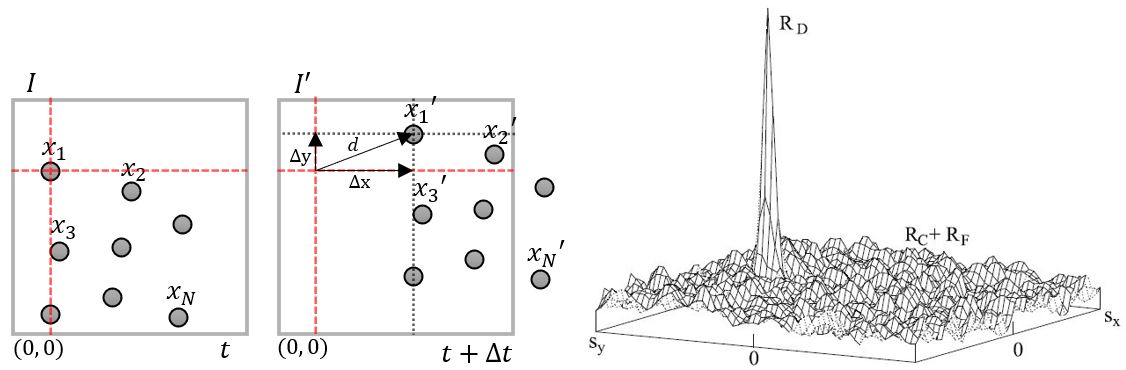
\includegraphics[width=16cm]{./3_MatPozadina/3_5KrosKorelacija.jpg} 
	\caption{Shema polja intenziteta $I$ i $I'$ u trenutcima $t$ i $t + \Delta t$ prikazana na prve dvije slike, te kompozicija vrhova korelacijske funkcije na trećoj slici \cite{raffel2018_book}}
	\label{sl:3.5}
\end{figure}
\par
Iz jednadžbe \ref{eqn:3.30} vidi se da pomak korelacije je funkcija nasumičnih varijabli $(\boldsymbol{X_{i}})_{i=1\dots N}$. Posljedično pomak je i sam nasumična varijabla i za različite izvedbe općenito istih uvjeta, dobit će se kvalitativno različite procjene pomaka koje ovise o stanju skupa čestica. Kako bi procjena pomaka u tom slučaju bila što bolja potrebno je izvesti pravila za generalnu optimizaciju procjene vrijednosti pomaka, što će biti prikazano u sljedećem poglavlju.
\FloatBarrier
\section{Očekivana vrijednost pomaka korelacije}
Kako bi se izvela pravila za opću procjenu pomaka odrediti će se očekivana vrijednost korelacijskog pomaka $E\{R_{D}\}$ za sve koncepte $\boldsymbol{\Gamma}$. Konkretnije, izračunati će se srednja korelacijska funkcija za sve moguće "uzorke" koji se mogu napraviti sa $N$ čestica. Iz jednadžbe \ref{eqn:3.30} slijedi:
\begin{equation}
	\begin{split}
		E\{R_{D}\} &= E\left\{R_{\tau}(\boldsymbol{s}-\boldsymbol{d})\sum_{i=1}^{N}V_{0}(\boldsymbol{X_{i}})\, V_{0}(\boldsymbol{X_{i}}+\boldsymbol{D})\right\}\\
		&=R_{\tau}(\boldsymbol{s}-\boldsymbol{d})\, E\left\{ \sum_{i=1}^{N}V_{0}(\boldsymbol{X_{i}})\, V_{0}(\boldsymbol{X_{i}}+\boldsymbol{D})\right\}
	\end{split}
	\label{eqn:3.31}
\end{equation}
Ako se zapiše $f_{l}(\boldsymbol{X})=V_{0}(\boldsymbol{X_{i}})\, V_{0}(\boldsymbol{X_{i}}+\boldsymbol{D})$:
\begin{equation*}
	E\{R_{D}\} = R_{\tau}(\boldsymbol{s}-\boldsymbol{d})\, E\left\{\sum_{i=1}^{N}f_{l}(\boldsymbol{X_{i}})\right\}
\end{equation*}
$\sum_{i=1}^{N}f_{l}(\boldsymbol{X_{i}})$ promatra se kao funkcija $N$ nasumičnih varijabli $\boldsymbol{X_{1}}, \boldsymbol{X_{2}},...\, \boldsymbol{X_{N}}$, te se zato može napisati:
\begin{equation}
	\begin{split}
		E\left\{\sum_{i=1}^{N}f_{l}(\boldsymbol{X_{i}})\right\} = \sum_{i=1}^{N}E\{f_{l}(\boldsymbol{X_{i}})\} = \sum_{i=1}^{N}\dfrac{1}{V_{F}}\int f_{l}(\boldsymbol{X_{i}})d\boldsymbol{X_{i}}\\
		\Rightarrow E\left\{\sum_{i=1}^{N}f_{l}(\boldsymbol{X_{i}})\right\} = \dfrac{N}{V_{F}}\int_{V_{F}}f_{l}(\boldsymbol{X})d\boldsymbol{X}
	\end{split}
	\label{eqn:3.32}
\end{equation}
gdje je $\int_{V_{F}} f_{l}(\boldsymbol{X})d\boldsymbol{X}$ volumenski integral
\begin{equation*}
	\int \int \int f_{l}(X, Y, Z)\, d\boldsymbol{X}d\boldsymbol{Y}d\boldsymbol{Z}
\end{equation*}
što konačno daje:
\begin{equation}
	E\{R_{D}\}= \dfrac{N}{V_{F}}R_{\tau}(\boldsymbol{s}-\boldsymbol{d})\int_{V_{F}}f_{l}(\boldsymbol{X})d\boldsymbol{X}
	\label{eqn:3.33}
\end{equation}
Kako je $N$ definiran kao ukupan broj svih čestica unutar fluida, tako i $V_{F}$ je interpretiran kao volumen fluida unutar kojeg su dodane čestice markeri. Prema gornjoj definiciji $f_{l}(\boldsymbol{X})$ u praktičnom smislu može se reći da integracija mora biti izvršena preko volumena koji se sastoji od volumena ispitivanja koji se nalaze na slikama dobivenim tijekom prve ili druge ekspozicije. Integral nad $f_{l}(\boldsymbol{X})$, drugim riječima može biti zapisan kao:
\begin{equation}
	\begin{split}
		\int_{V_{F}}f_{l}(\boldsymbol{X})d\boldsymbol{X}  &= \int I_{0}(Z)\, I_{0}(Z+D_{Z})dZ \times \int \int W_{0}(X,Y)\, W_{0}(X+D_{X},Y+D_{Y})dXdY \\
		&=\int_{V_{F}}V_{0}^{2}(\boldsymbol{X})d\boldsymbol{X}\dot F_{O}(D_{Z})F_{I}(D_{X},D_{Y})
	\end{split}
	\label{eqn:3.34}
\end{equation}
gdje su:
\begin{equation}
	F_{I}(D_{X},D_{Y})=\dfrac{\int \int W_{0}(X, Y)\, W_{0}(X+D_{X}, Y+D_{Y})dXdY}{\int \int W_{0}^{2}(X, Y)dXdY}
	\label{eqn:3.35}
\end{equation}
i
\begin{equation}
	F_{O}(D_{Z})=\dfrac{\int I_{0}(Z)\, I_{0}(Z+D_{Z})dZ}{\int I_{0}^{2}(Z)dZ}
	\label{eqn:3.36}
\end{equation}
Prema literaturi \cite{keane1992theory} $F_{I}$ je definiran kao faktor koji izražava unutar-ravninski gubitak parova. Konačno jednadžba \ref{eqn:3.33} ima oblik:
\begin{equation}
	E\left\{R_{D}(\boldsymbol{s}, \boldsymbol{D})\right\}=C_{R}R_{\tau}(\boldsymbol{s}-\boldsymbol{d})F_{O}(D_{Z})F_{I}(D_{X},D_{Y})
	\label{eqn:3.37}
\end{equation}
gdje je konstanta $C_{R}$ definirana kao:
\begin{equation*}
	C_{R}=\dfrac{N}{V_{F}}\int_{V_{F}}V_{0}^{2}(\boldsymbol{X})d\boldsymbol{X}
\end{equation*}
U 2D PIV-u gubitak korelacije zbog gibanja izvan ravnine ili neusklađenosti svjetlosne ravnine ima dva efekta. Prvi efekt je u tome da je smanjena vjerojatnost detekcije ispravnog vektora brzina. Drugo, povećana je nesigurnost u mjerenjima polja brzina. Valjanost originalne definicije $F_{O}$ prema \cite{keane1992theory} je limitirana na upotrebu identičnog intenziteta laserskog profila pri svakoj ekspoziciji. Kako se laserska ravnina prilikom prvog i drugog osvijetljenja obično razlikuje u širini i obliku, korištenje predložene definicije $F_{O}$ je limitirano u praksi. Kako bi se zaobišla ova limitacija, u literaturi \cite{scharnowski2017generalization} predložena je nova definicija $F_{O}$ koja točno predviđa gubitak korelacije za sve neusklađene svjetlosne ravnine, te također potvrđuje originalnu $F_{O}$ definiciju prilikom idealnih uvjeta. 